\documentclass[a0paper,portrait,fontscale = 0.32,margin=1.5em]{baposter/baposter}

\usepackage{relsize}
\usepackage{url}
\usepackage{amsmath}
\usepackage{bm}
\usepackage{setspace}
\usepackage[utf8x]{inputenc}
\usepackage{multicol}

%%% Global Settings %%%%%%%%%%%%%%%%%%%%%%%%%%%%%%%%%%%%%%%%%%%%%%%%%%%%%%%%%%%

\graphicspath{{pix/}}	% Root directory of the pictures
\tracingstats=2			% Enabled LaTeX logging with conditionals

%%% Color Definitions %%%%%%%%%%%%%%%%%%%%%%%%%%%%%%%%%%%%%%%%%%%%%%%%%%%%%%%%%
\definecolor{bordercol}{RGB}{40,40,40}
\definecolor{headercol1}{RGB}{186,215,230}
\definecolor{headercol2}{RGB}{80,80,80}
\definecolor{headerfontcol}{RGB}{0,0,0}
\definecolor{boxcolor}{RGB}{186,215,230}
\definecolor{sublue}{RGB}{0,47,95}
\definecolor{suorange}{RGB}{235,113,37}
\definecolor{suoliv}{RGB}{163,168,107}
\definecolor{sulightblue}{RGB}{155,178,206}
\definecolor{sucyan}{RGB}{161,216,224}

\newcommand{\compresslist}{
	\setlength{\itemsep}{1pt}
	\setlength{\parskip}{0pt}
	\setlength{\parsep}{0pt}
}

\begin{document}

\typeout{Poster rendering started}

%%% Setting Background Image %%%%%%%%%%%%%%%%%%%%%%%%%%%%%%%%%%%%%%%%%%%%%%%%%%
% \background{
% 	\begin{tikzpicture}[remember picture,overlay]%
% 	\draw (current page.north west)+(-2em,2em) node[anchor=north west]
% 	{\includegraphics[height=1.1\textheight]{background}};
% 	\end{tikzpicture}
% }

%%% General Poster Settings %%%%%%%%%%%%%%%%%%%%%%%%%%%%%%%%%%%%%%%%%%%%%%%%%%%
%%%%%% Eye Catcher, Title, Authors and University Images %%%%%%%%%%%%%%%%%%%%%%
\begin{poster}{
    grid=false,
    % Option is left on true though the eyecatcher is not used. The reason is
    % that we have a bit nicer looking title and author formatting in the headercol
    % this way
    eyecatcher=false,
    headerColorOne=suorange,
    borderColor=white,
    headerColorTwo=suoliv,
    headerFontColor=white,
    % Only simple background color used, no shading, so boxColorTwo isn't necessary
    boxColorTwo=sulightblue,
    boxColorOne=white,
    headershape=roundedright,
    headerfont=\Large\sf\bf,
    textborder=roundedleft,
    headerborder=open,
    boxshade=plain,
    %%%%%%%
    bgColorOne=sublue,
    bgColorTwo=suoliv,
    background=shadelr
}
  %%% Eye Cacther %%%%%%%%%%%%%%%%%%%%%%%%%%%%%%%%%%%%%%%%%%%%%%%%%%%%%%%%%%%%%%%
{
  %Eye Catcher, empty if option eyecatcher=false - unused
}
%%% Title %%%%%%%%%%%%%%%%%%%%%%%%%%%%%%%%%%%%%%%%%%%%%%%%%%%%%%%%%%%%%%%%%%%%%
{\sf \bf \Huge
{\color{white} \Huge \textbf{Efficient Bayesian Multivariate Surface Regression}}
}
%%% Authors %%%%%%%%%%%%%%%%%%%%%%%%%%%%%%%%%%%%%%%%%%%%%%%%%%%%%%%%%%%%%%%%%%%
{
{\color{suorange} {\newline  \sc Feng Li, Department of Statistics, Stockholm University, Sweden}\\[0.50em]
  \sc Mattias Villani,  Division of Statistics at Linköping University}
}
%%% Logo %%%%%%%%%%%%%%%%%%%%%%%%%%%%%%%%%%%%%%%%%%%%%%%%%%%%%%%%%%%%%%%%%%%%%%
{
% The logos are compressed a bit into a simple box to make them smaller on the result
% (Wasn't able to find any bigger of them.)
\setlength\fboxsep{0pt}
\setlength\fboxrule{0.0pt}
	\fbox{
          \begin{minipage}{10em}
            \includegraphics[height=9.5em]{Stockholm_University_logo}
          \end{minipage}
	}
      }

\headerbox{Contributions}{name=problem,column=0,row=0}
{

  We propose a regression model for a multivariate Gaussian response that
  combines both additive splines and interactive splines, and a highly
  efficient MCMC algorithm that updates all the multivariate knot locations
  jointly. We use shrinkage priors to avoid overfitting with different
  estimated shrinkage factors for the additive and surface part of the model,
  and also different shrinkage parameters for the different response variables.

}

\headerbox{The model}{name=definitions,column=0,below=problem}{

  The multivariate surface model consists of three components,
    {\color{red}\emph{\textbf{linear}}}, {\color{red}\emph{\textbf{surface}}} and
    {\color{red}\emph{\textbf{additive}}} as
    \[\begin{gathered}
      \bm{Y}=\bm{X}_o\bm{B}_o+
      \bm{X}_s(\bm{\xi}_s)\bm{B}_s+\bm{X}_a(\bm{\xi}_a)\bm{B}_a + \bm{E}
    \end{gathered}\] where
    ${\bm{x}_{sj}(\bm{\xi}_{sj})}=\Vert\bm{x}_{o}-\bm{\xi}_{sj}\Vert^{2}\ln\Vert\bm{x}_{o}-\bm{\xi}_{sj}\Vert$,
    for $j=1, ..., q_s$ are the surface thin-plate bases. The univariate
    thin-plate basis ${\bm{x}_{aj}(\bm{\xi}_{aj})}$ used in the additive part
    is a special case of the multivariate thin-plate in where both the data
    point and the knot are one-dimensional. We treat the knots $\bm{\xi}_i$ as
    unknown parameters and let them move jointly.

  % {\smaller {\color{red} $\bullet$} We treat the knots $\xi_i$ as unknown parameters and let them move
  %   jointly.\\
  % {\color{red} $\bullet$} We found a model with a minimal number of free knots outperforms
  % model with lots fixed knots.}
}

\headerbox{The shrinkage prior}{name=models,column=0,below=definitions}{

  Conditional on $\bm{\xi}$, the prior for $\bm{B}$ and $\bm{\Sigma}$ are set as
    \[
    \begin{split} \mathrm{vec}\bm{B}_i |\bm{\Sigma},~\bm{\lambda}_i &\sim
\bm{N}_q\left( \mu _i, ~\bm{\Lambda}_i^{1/2} \bm{\Sigma} \bm{\Lambda}_i^{1/2}
\otimes \bm{P}_i^{-1} \right),\\ \bm{\Sigma} &\sim
\bm{IW} \left(n_0 \bm{S}_0,~n_0\right), ~i\in \{o,s,a \},
    \end{split}
    \] where
$\bm{\Lambda}_i=diag(\bm{\lambda}_i)$ are the shrinkage
parameters, which is used to overcome overfitting.

{\smaller {\color{red} $\bullet$} The shrinkage parameters are estimated by MCMC. A small
$\bm{\lambda}_{i}$ shrinks the variance of the conditional posterior for
$\bm{B}_i$. \\
{\color{red} $\bullet$} The priors for knots are from multivariate normal
distribution where the means are set through \emph{k}-means clustering.}

% {\color{red} $\bullet$} We allow for mixing use different settings of $\bm{P}_i$ in different components.}

}

\headerbox{The posterior inference}{name=inference,column=0,below=models}{

The posterior distribution $p(\bm{B},\bm{\Sigma},\bm{\xi},\bm{\lambda}|\bm{Y},\bm{X})$ is conveniently decomposed as
    \[ p(\bm{B}|\bm{\Sigma},\bm{\xi},\bm{\lambda},\bm{Y},\bm{X})p(\bm{\Sigma}|\bm{\xi},\bm{\lambda},\bm{Y},\bm{X})p(\bm{\xi},\bm{\lambda}|\bm{Y},\bm{X}).
    \]

where the coefficients ($\bm{B}$) can be integrated out analytically. We
  update covariance ($\bm{\Sigma}$), all knots ($\bm{\xi}$) and shrinkages
  ($\bm{\lambda}$) jointly by using Metropolis-Hastings within Gibbs.

  {\smaller {\color{red} $\bullet$} The proposal density for $\bm{\xi}$ and $\bm{\lambda}$ is a multivariate \emph{t}-density with $\nu>2$ df,
      \[
      \bm{\theta}_{p}|\bm{\theta}_{c}\sim\bm{MVT}\left[\bm{\hat{\theta}},~\left.-\left(\frac{\partial^{2}\ln
              p(\bm{\theta}|\bm{Y})}{\partial\bm{\theta}\partial\bm{\theta}^{\prime}}\right)^{-1}\right\vert
        _{\bm{\theta}=\bm{\hat{\theta}}},~\nu\right],
      \] where $\bm{\hat{\theta}}$ is obtained by $k$ steps ($k\leq 3$) Newton's
        iterations during the proposal with analytical gradients for matrices.\\
    {\color{red} $\bullet$}  The proposal density for $\bm{\Sigma}$ is the inverse Wishart
      density.}
}

\headerbox{Remarks}{name=compremark,column=0,below=inference}{

  An important feature of our algorithm is that all knot locations are sampled
  jointly using a Metropolis-Hastings proposal density tailored to the
  conditional posterior, rather than the \emph{one-knot-at-a-time} random walk
  proposals used in previous literature.

  {\smaller {\color{red} $\bullet$} An efficient realization requires great
    care of the sparsity problem and the analytical gradient w.r.t. unknown
    parameters, though it is straightforward to implement the MCMC algorithm.}

  {\smaller {\color{red} $\bullet$} It is possible to generalize the model and MCMC to
  Non-Gaussian responses and to augment the shrinkage with variable selection.}
}

\headerbox{Footnotes}{name=acknowledgements,column=0,below=compremark}{

\begin{spacing}{0.70}
  {\tiny Li ({\color{red}{\texttt{feng.li@stat.su.se}}}) is Ph.D student of
    Statistics at Stockholm University. Villani
    ({\color{red}{\texttt{mattias.villani@liu.se}}}) is Professor of Statistics
    at the Division of Statistics of the Department of Computer and Information
    Science at Linköping University. The authors are grateful to Paolo Giordani
    and Robert Kohn for stimulating discussions and constructive suggestions.

    A preprint of this paper is available at \textbf{\color{red}{\url{http://arxiv.org/abs/1110.3689}}}.}
  \end{spacing}
}

\headerbox{The simulation study}{name=density,span=2,column=1,row=0}{

   \begin{multicols}{3}

{\color{red} \textbf{DGP:}}
We randomly generate multivariate surface datasets with various degrees of nonlinearity.\\
{\color{red} \textbf{Estimation:}} We fit each dataset with the fixed knots
model with $5$, $10$, $15$, $20$, $25$ and $50$ surface knots, and also the free
knots model with $5$, $10$, and $15$ surface knots.

{\color{red} \textbf{Results:}} The free knots model outperforms the fixed knots
     model in the large majority of the datasets which is particularly true
     when the data are strongly nonlinear (Figures: example results for $p=2$, $n = 200$).

     \newpage
     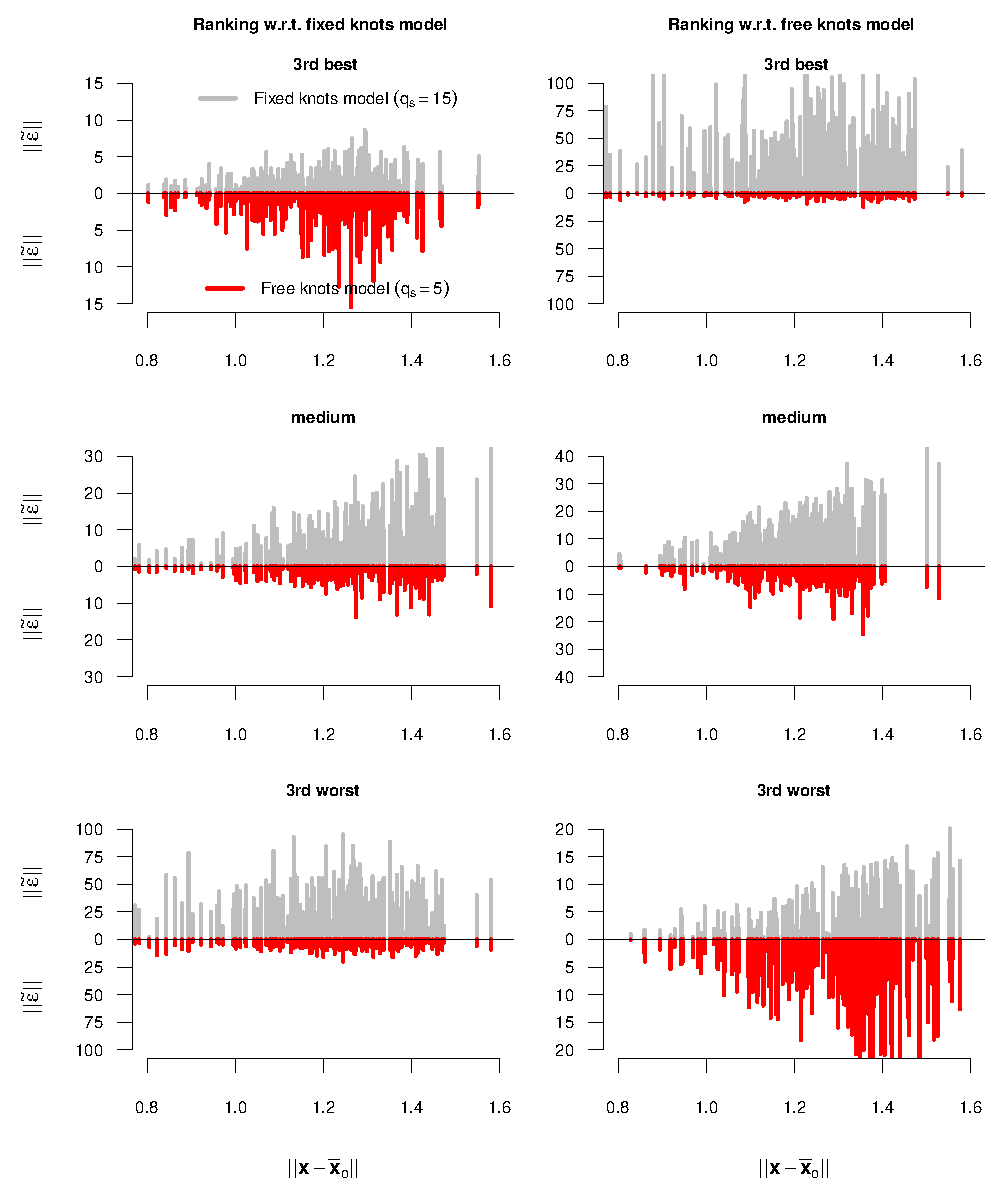
\includegraphics[width=0.32\textwidth]{SimResidPlot.eps}\newpage
     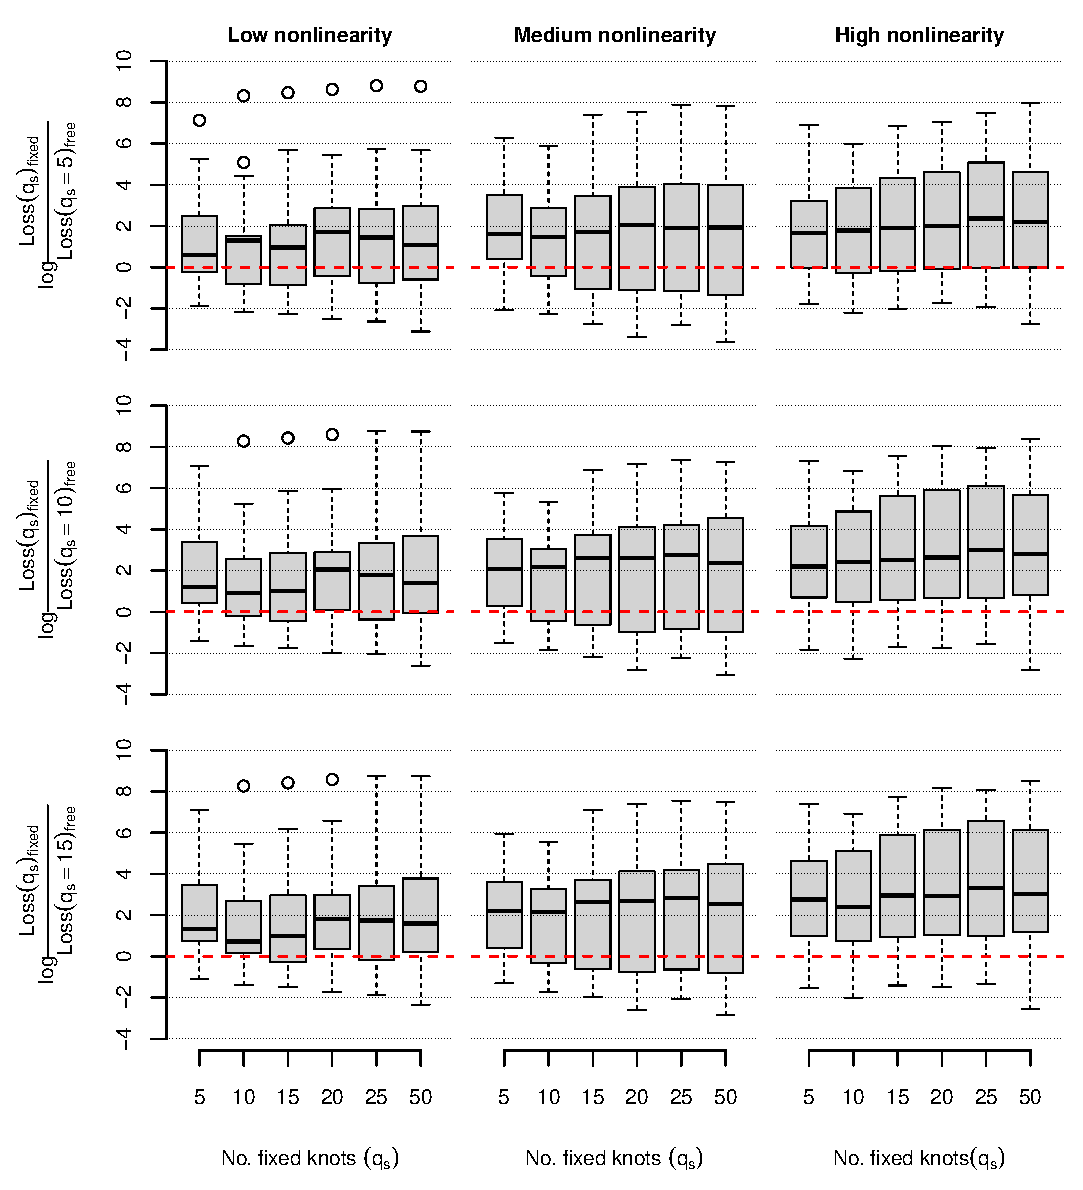
\includegraphics[width=0.32\textwidth]{LOSS_p2.eps}
\end{multicols}


 }

\headerbox{The firm leverage data application}
{name=simulation,span=2,column=1,below=density}{
  \scalebox{0.80}{
    \begin{tabular}{l|rl}
    {\color{red} Response} & \textbf{Leverage ($Y$):} &total debt/(total debt + book value of equity),
      for American
      non-financial $4405$ firms in $1992$\\
\hline
    {\color{red} Covariates} & \textbf{Tang:} & tangible assets/book value of total assets\\
     & \textbf{Market2Book:} &(book value of total assets - book value of equity +
      market value of equity) / book value of total assets\\
     & \textbf{LogSales:} &logarithm of sales\\
     & \textbf{Profit:} &(earnings before interest, taxes, depreciation, and amortization) /
      book value of total assets    \\
    \end{tabular}}
  \begin{center}
    \includegraphics[width=1\textwidth]{Rajanscatter2}\\
  \end{center}

\begin{multicols}{3}

{\color{red} \textbf{Out-of-sample comparison:\\}}
We compare and select models based on the $D$-fold
out-of-sample log predictive density score (LPDS) which is defined as
\[
\begin{split}
&\frac{1}{D}\sum\limits_{d=1}^{D}\ln p(\tilde{\bm{Y}}_{d}|\tilde{\bm{Y}}_{-d},\bm{X}),\\
\end{split}
\]
where the predictive density is $\int\!\prod\nolimits_{i\in\tau_{d}}p(\bm{y}_{i}|\bm{\theta},
\bm{x}_{i})p(\bm{\theta}|\tilde{\bm{Y}}_{-d})\mathrm{d}\bm{\theta}$ and
$\tilde{\bm{Y}}_{d}$ is an $(n_{d}\times p)$ matrix containing the $n_{d}$
observations in the $d$th testing sample and $\tilde{\bm{Y}}_{-d}$ denotes the
training observations used for estimation. We assume that the observations
are independent. The main advantage for choosing LPDS instead of the marginal
likelihood is that the LPDS is not sensitive to the choice of prior.

{\color{red} \textbf{Findings:\\}}
  {\smaller {\color{red} $\bullet$} We find a model with a minimal number of free knots outperforms
  model with many fixed knots.}

% conditional on $\bm{\theta}$,
% then
% % \[
% % p(\tilde{\bm{Y}}_{d}|\tilde{\bm{Y}}_{-d},
% % \bm{X})=\int\!\prod\nolimits_{i\in\tau_{d}}p(\bm{y}_{i}|\bm{\theta},
% % \bm{x}_{i})p(\bm{\theta}|\tilde{\bm{Y}}_{-d})\mathrm{d}\bm{\theta},
% % \]
% where $\tau_{d}$ is the index set for the observations in $\tilde{\bm{Y}}_{d}$,
% and the LPDS is easily computed by averaging
% $\prod_{i\in\tau_{d}}p(\bm{y}_{i}|\bm{\theta}, \bm{x}_{i})$ over the posterior
% draws from $p(\bm{\theta}|\tilde{\bm{Y}}_{-d})$.
\newpage
     % {\color{red} $\rightarrow$} {\smaller Models with both additive and
     %    surface components}\\
     %  {\color{red} $\downarrow$} {\smaller Models with only surface or additive components
     %    components.}
    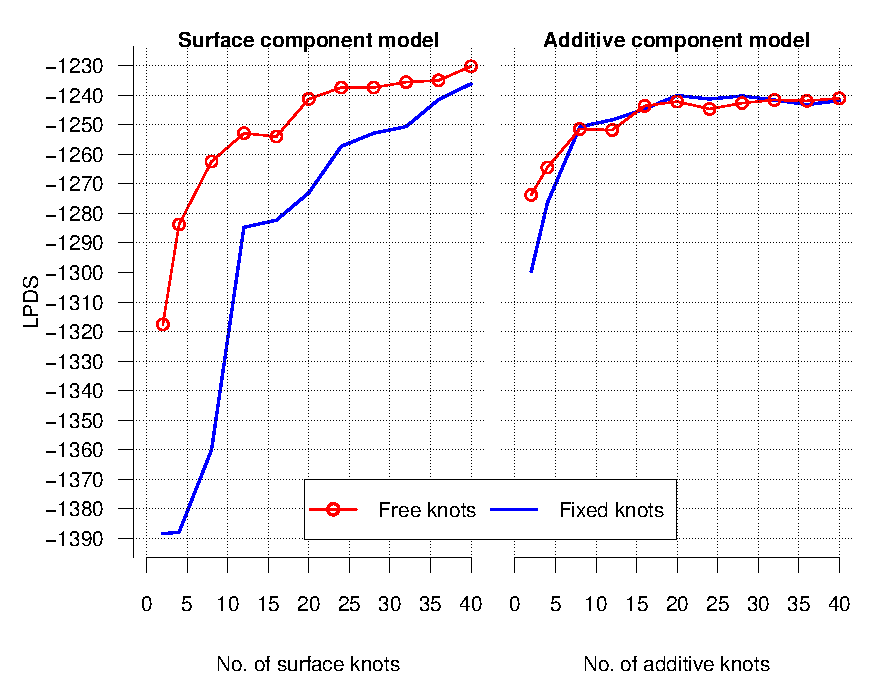
\includegraphics[width=0.32\textwidth]{RajanLPDS_SurfaceBesideAdditive}

{\smaller {\color{red} $\bullet$}
The free knots model always outperforms the fixed knots model when only
a surface component is used.\\
}
{\smaller {\color{red} $\bullet$}
The ability to
move the knots clearly also helps to keep the number of knots to a minimum,
which is crucial in high dimensional data.\\
}
{\smaller {\color{red} $\bullet$}
There are generally
improvements from using both surface knots and additive knots in the same
model.\\
}
{\smaller {\color{red} $\bullet$}
The shrinkage prior is very effective in
mitigating potential problems with overfitting.\\
}

\newpage 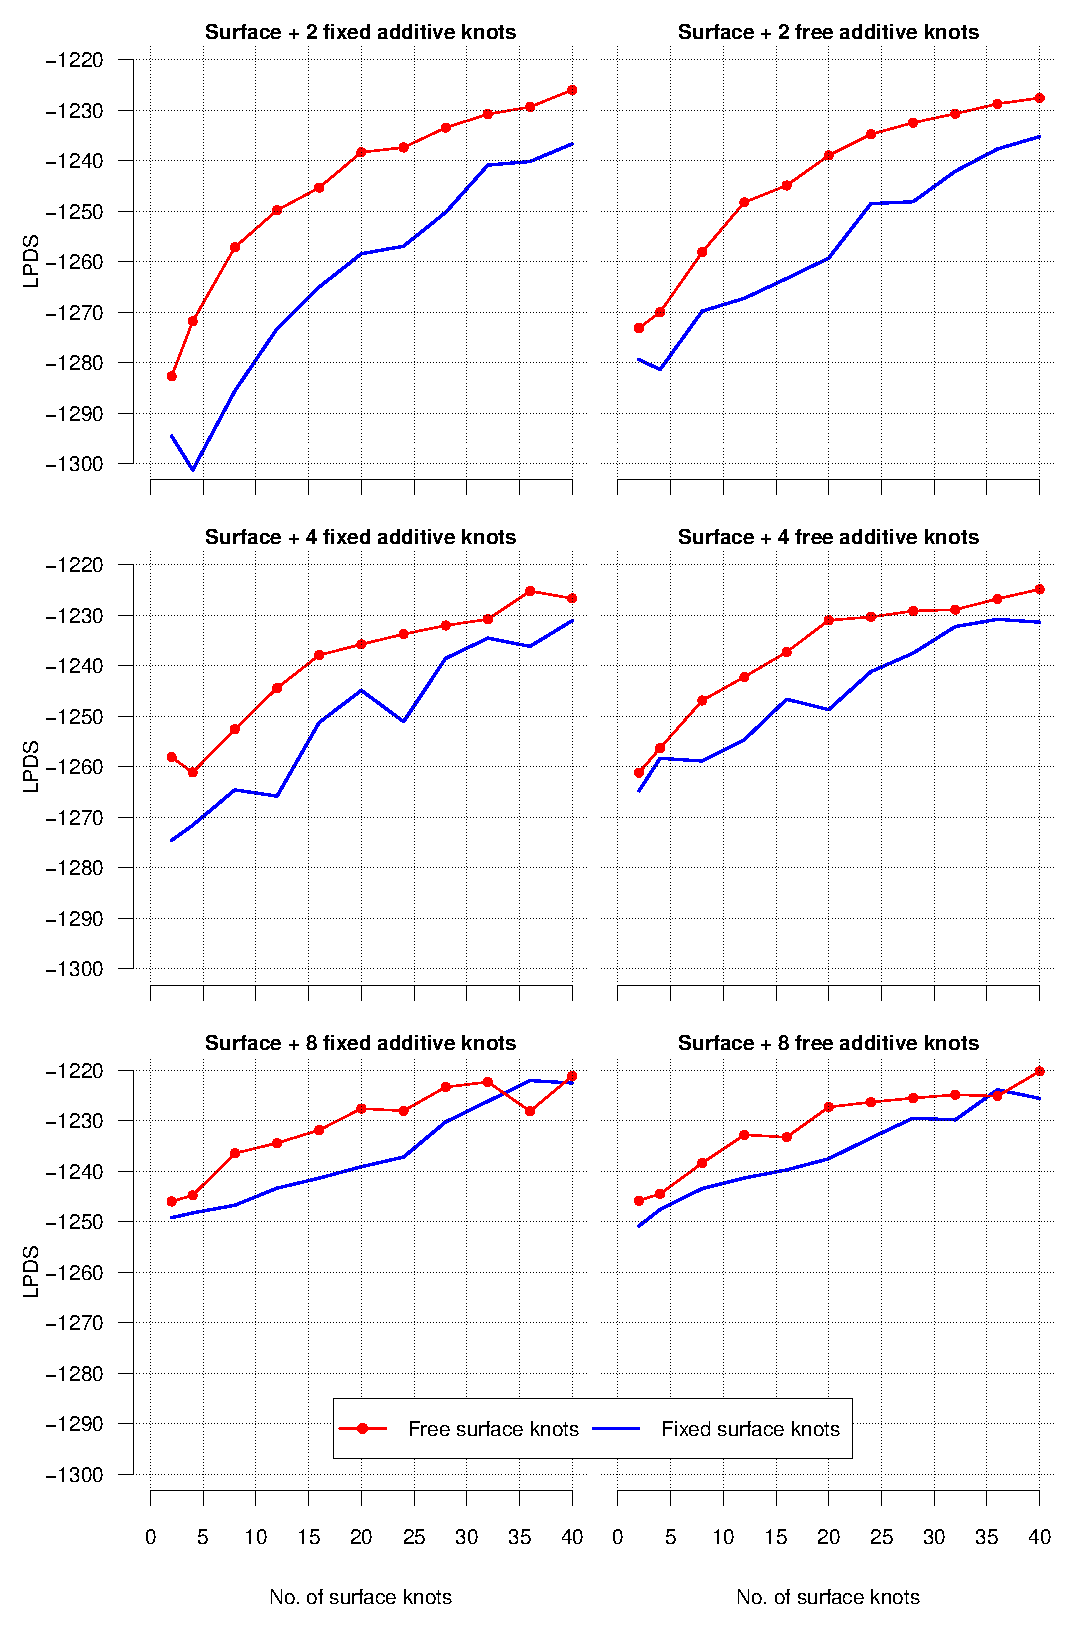
\includegraphics[width=0.32\textwidth]{RajanLPDS_SurfacePlusAdditive}

{\smaller {\color{red} $\bullet$}
The free knots model is also more robust in the sense that it performs
consistently well across models with different numbers of knots.
}
\end{multicols}

\begin{multicols}{3}

  {\color{red} \textbf{Posterior presentation:\\}}
We use heat map to visualize
  the posterior density of the knot locations in covariate space (bottom
  left). Because of the \emph{knot switching problem}, it does not make much
  sense to display the posterior distribution of the knot locations
  directly. We present the posterior mean (bottom middle) and standard
  deviation (bottom right) of the posterior surface for the model with $4$ free
  additive knots and $20$ free surface knots for firm leverage data with
  covariates. It also plots the covariate observations to give a sense of where
  the data observations are located.

\end{multicols}

\begin{center}  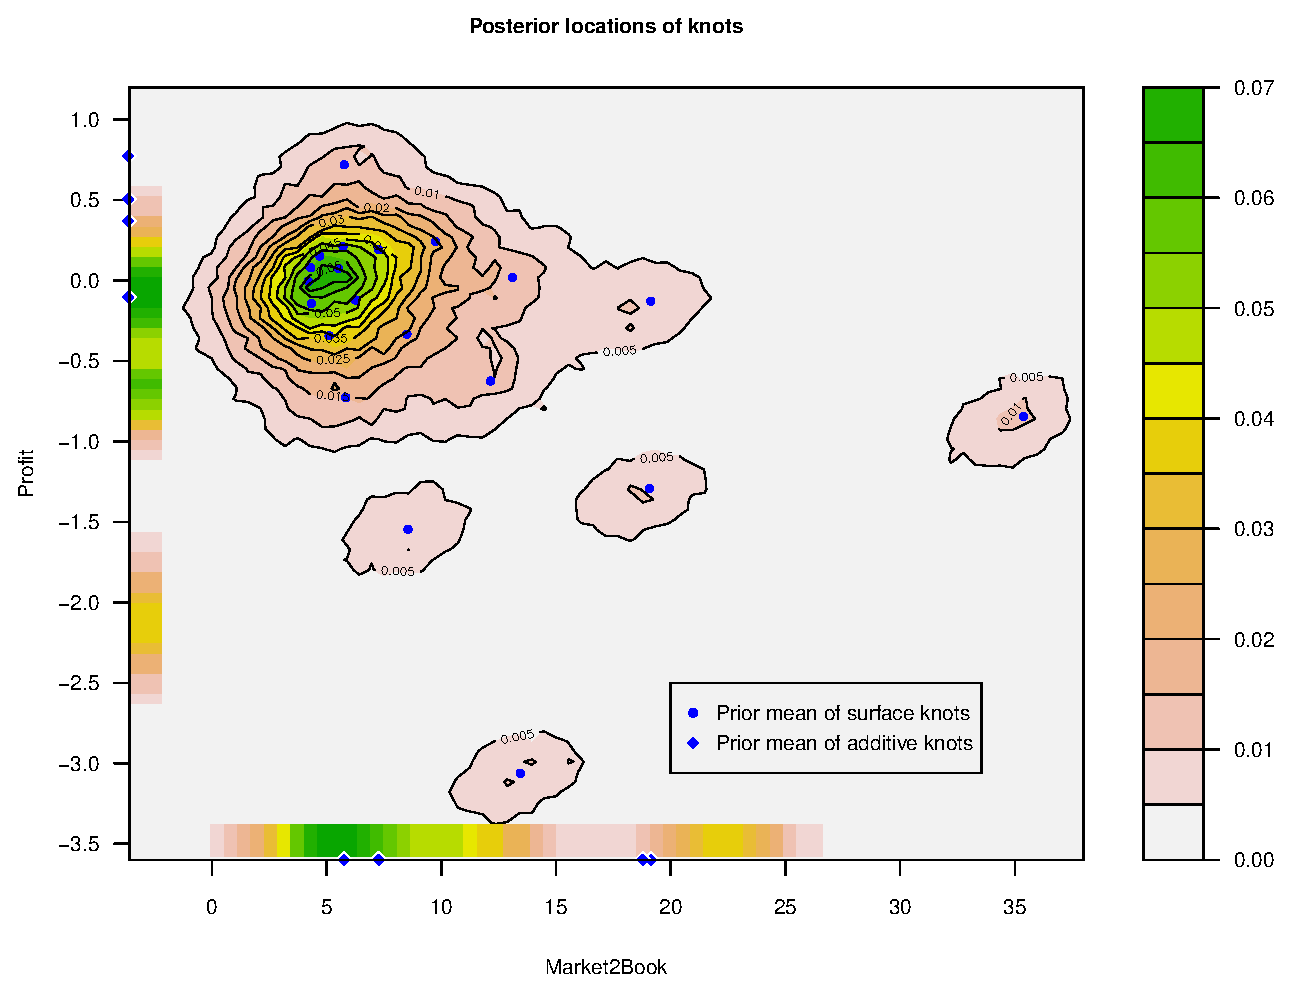
\includegraphics[width=0.33\textwidth]{RajanPostKnots.eps}\hspace{0.2em}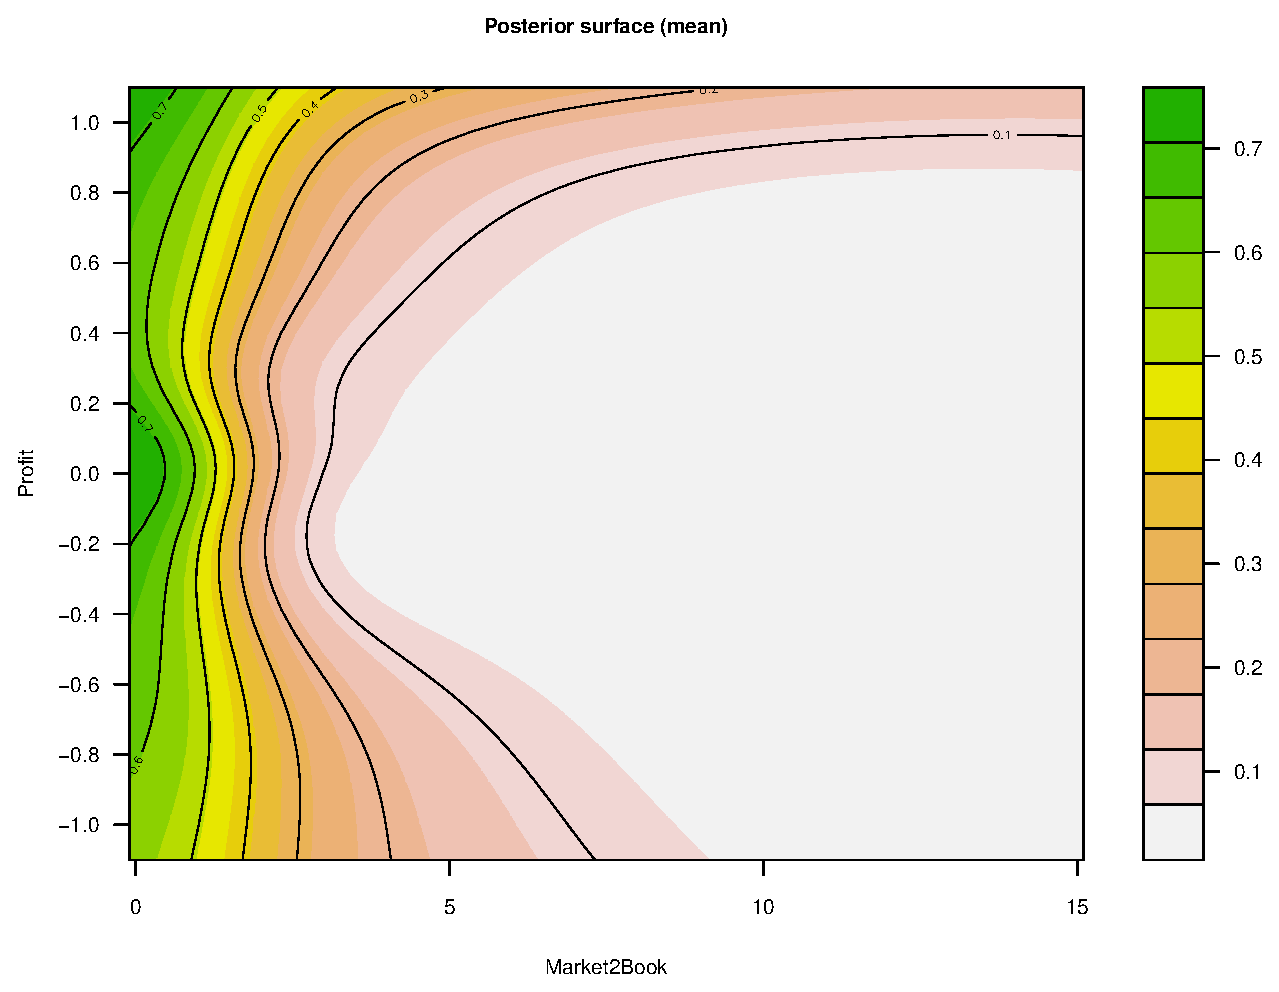
\includegraphics[width=0.33\textwidth]{RajanPostMean.eps}\hspace{0.2em}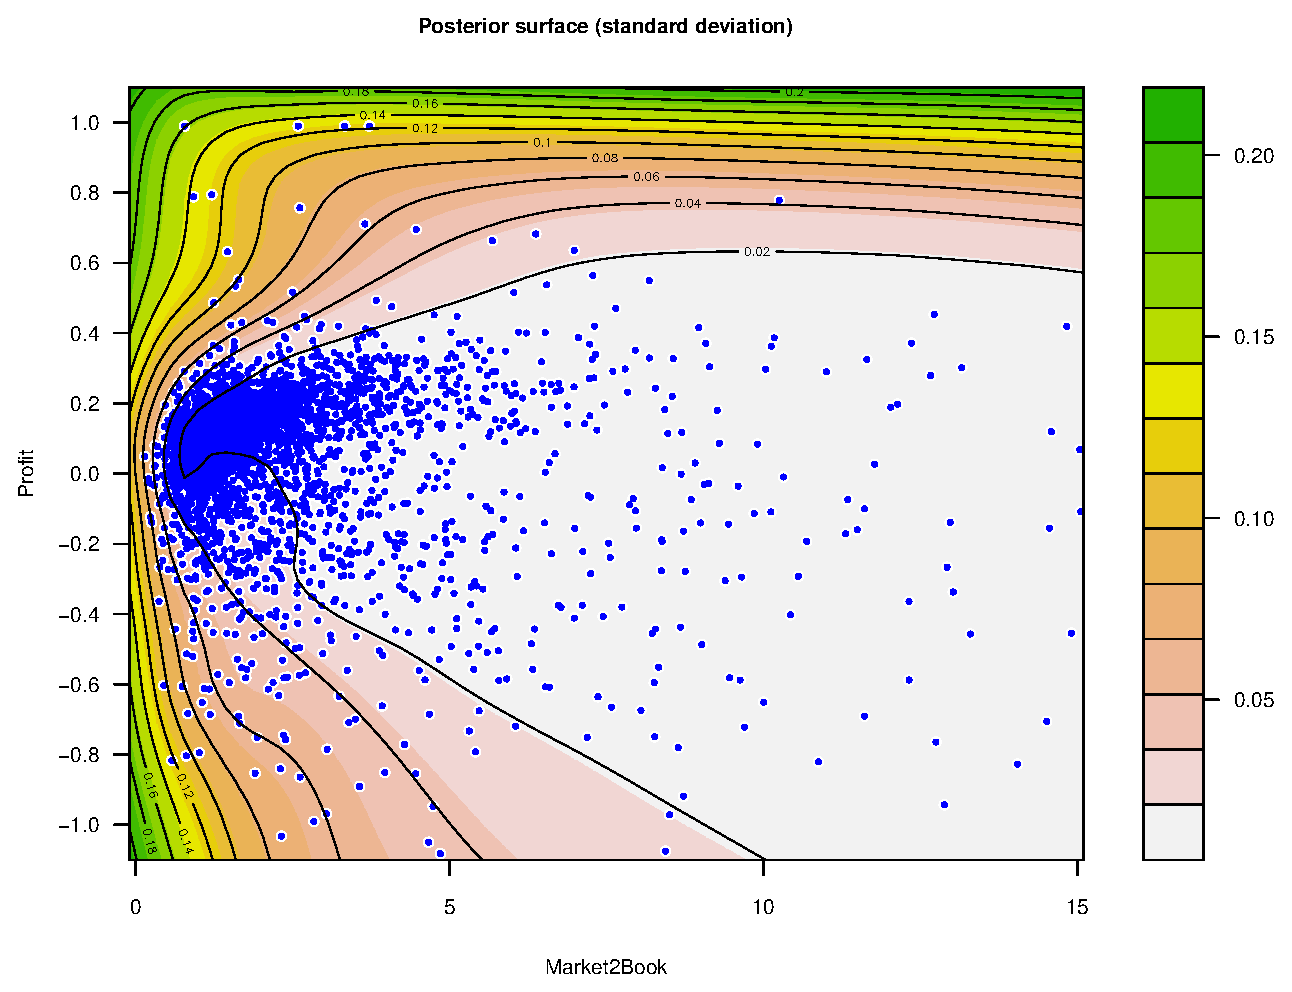
\includegraphics[width=0.33\textwidth]{RajanPostSD.eps}
  \end{center}

}


% \headerbox{The firm leverage data application}
% {name=leverage,span=2,column=1,below=simulation}{
% }

\end{poster}
\end{document}